% Journal Article
% LaTeX Template
% Version 1.4 (15/5/16)
%
% This template has been downloaded from:
% http://www.LaTeXTemplates.com
%
% Original author:
% Frits Wenneker (http://www.howtotex.com) with extensive modifications by
% Vel (vel@LaTeXTemplates.com)
%
% License:
% CC BY-NC-SA 3.0 (http://creativecommons.org/licenses/by-nc-sa/3.0/)
%
%%%%%%%%%%%%%%%%%%%%%%%%%%%%%%%%%%%%%%%%%

%----------------------------------------------------------------------------------------
%	PACKAGES AND OTHER DOCUMENT CONFIGURATIONS
%----------------------------------------------------------------------------------------

\documentclass[twoside,twocolumn]{article}

\usepackage{blindtext} % Package to generate dummy text throughout this template 
\usepackage{graphicx}
\usepackage{subfig}
\usepackage[sc]{mathpazo} % Use the Palatino font
\usepackage[T1]{fontenc} % Use 8-bit encoding that has 256 glyphs
\linespread{1.05} % Line spacing - Palatino needs more space between lines
\usepackage{microtype} % Slightly tweak font spacing for aesthetics

\usepackage[spanish]{babel} % Language hyphenation and typographical rules

\usepackage[hmarginratio=1:1,top=32mm,columnsep=20pt]{geometry} % Document margins
\usepackage[hang, small,labelfont=bf,up,textfont=it,up]{caption} % Custom captions under/above floats in tables or figures
\usepackage{lettrine} % The lettrine is the first enlarged letter at the beginning of the text

\usepackage{enumitem} % Customized lists
\setlist[itemize]{noitemsep} % Make itemize lists more compact


\usepackage{titlesec} % Allows customization of titles
\renewcommand\thesection{\Roman{section}} % Roman numerals for the sections
\renewcommand\thesubsection{\roman{subsection}} % roman numerals for subsections
\titleformat{\section}[block]{\large\scshape\centering}{\thesection.}{1em}{} % Change the look of the section titles
\titleformat{\subsection}[block]{\large}{\thesubsection.}{1em}{} % Change the look of the section titles

\usepackage{fancyhdr} % Headers and footers
\pagestyle{fancy} % All pages have headers and footers
\fancyhead{} % Blank out the default header
\fancyfoot{} % Blank out the default footer
\fancyhead[C]{Anteproyecto $\bullet$ Diciembre de 2021} % Custom header text
\fancyfoot[RO,LE]{\thepage} % Custom footer text
\fancyfoot[C]{Ramón Serrano Fernández}
\usepackage{titling} % Customizing the title section

\usepackage{hyperref} % For hyperlinks in the PDF

%----------------------------------------------------------------------------------------
%	TITLE SECTION
%----------------------------------------------------------------------------------------

\setlength{\droptitle}{-4\baselineskip} % Move the title up

\pretitle{\begin{center}\Huge\bfseries} % Article title formatting
\posttitle{\end{center}} % Article title closing formatting
\title{Anteproyecto} % Article title
\author{%
\textsc{Ramón Serrano} \\[1ex] % Your name
\normalsize Universidad de Salamanca \\ % Your institution
\normalsize \href{mailto:rserranof03@usal.es}{rserranof03@usal.es} % Your email address
%\and % Uncomment if 2 authors are required, duplicate these 4 lines if more
%\textsc{Jane Smith}\thanks{Corresponding author} \\[1ex] % Second author's name
%\normalsize University of Utah \\ % Second author's institution
%\normalsize \href{mailto:jane@smith.com}{jane@smith.com} % Second author's email address
}
\date{\today} % Leave empty to omit a date
\renewcommand{\maketitlehookd}{%
}

%----------------------------------------------------------------------------------------

\begin{document}

% Print the title
\maketitle

%----------------------------------------------------------------------------------------
%	ARTICLE CONTENTS
%----------------------------------------------------------------------------------------

\section{Idea Inicial y Evolución del proyecto
pictórico\label{idea-inicial-y-evoluciuxf3n-del-proyecto-pictuxf3rico}}

\lettrine[nindent=0em,lines=3]{L}a idea inicial de este proyecto fue, sobre todo, la de crear un mundo
fantástico y una mitología propia, del que poder partir para hablar de
diversos temas que siempre me han interesado. Los temas en que quería
centrarme eran mayormente la \textbf{decadencia}, la \textbf{juventud} y
lo \textbf{onírico}. Otros temas que prentendía tratar y que creo que al
final no han resultado plasmados eran la \textbf{herencia} y la
\textbf{apropiación de los espacios}.

Los referentes principales en los que me inspiré fueron: Turner, de
quien me interesa sobre todo el uso del color y la pseudo abstracción,
Kaspar David Friederich, en quien encuentro muy inspiradores los
paisajes de ruinas desolados, William Blake y Alan Lee, por parte de las
artes plásticas y J. R. R. Tolkien y Brandon Sanderson por parte de la
escritura, maestros de la fantasía y creadores de mundos, Neil Gaimann
(escritor) y El Bosco, que crean mundos fantásticos y extremadamente
extraños. Además de muchos clásicos, tanto de la pintura como de la
literatura, como Dante, Leonardo, Velázquez, Goya o Durero.

Todo esto queda plasmado en el mapa conceptual en el que se ha
convertido mi esquina del
taller.

\begin{figure*}
  \centering
  \includegraphics[scale=0.2]{/Users/rserrano/grepos/ProyectoFinal/WhatsApp Image 2021-10-18 at 15.56.06.jpeg}
  \caption{Panorámica de la Esquina}
\end{figure*}

\begin{figure*}
  \centering
  \includegraphics[scale=0.05]{/Users/rserrano/grepos/ProyectoFinal/IMG_20211014_162123-1.jpg}
  \caption{Detalles del mapa conceptual en la Esquina (a octubre de 2021)}
\end{figure*}

\begin{center}\rule{0.5\linewidth}{0.5pt}\end{center}

La evolución de este cúmulo de ideas iniciales ha ideo tendiendo a lo
largo del cuatrimestre, generalmente, a una simplificación, no de los
conceptos a tratar, sino de la complejidad semántica de cada obra, desde
el primer proyeto sobre la sinéctica, en el que desarrollé una
simbología y un transfondo complejos, que trataban la mayoría de los
puntos establecidos en el mapa, hasta el último, sobre los no lugares,
en el que, sin perder complejidad material y plástica, la idea de un la
representación de un lugar agreste y hostil era mucho más directa y
sencilla, y se relacionaba con los demás pilares del proyecto de manera
órganica e implícita, en vez de explícita y simbólica.

\hypertarget{marco-teuxf3rico}{%
\subsection{Marco Teórico}\label{marco-teuxf3rico}}

Para la creación de este mundo fantástico propio, la principal fuente de
inspiración y de información sobre el propio procedimiento de creación
de estos mundos son autores del ámbito de la escritura. Como ya he
citado antes, dos de mis escritores favoritos y en cuyos métodos me baso
son J.R.R. Tolkien y Brandon Sanderson. Desde hace unos años existen
muchos recursos, Sobre todo en internet, que hablan de
\emph{worldbuilding}, construcción de mundos, y las técnicas que
conviene emplear. Brandon Sanderson incluso da clases universitarias
sobre este tema.

Más alejado del campo práctico de la creación de mundos, son
interesantes las visiones históricas de la fantasía y el folklore, y los
conceptos filosóficos de lo \emph{maravilloso} y lo \emph{sublime}.

Sin embargo, en cuanto al tratamiento de los temas y al enfoque del
proyecto, no creo que tenga una base teórica extremadamente
desarrollada, pues creo que habla sobre todo de mí, y parte más de la
emoción que de la reflexión.

\hypertarget{metodologuxeda-de-trabajo}{%
\subsection{Metodología de trabajo}\label{metodologuxeda-de-trabajo}}

La metodología de trabajo empleada para desarrollar el proyecto ha ido
cambiando a medida que desarrollaba las diferentes obras.

En los primeros trabajos, las ideass surgían más lentamente, y la
mayoría de las veces, sin reflexionar mucho, una de las primeras
composiciones o ideas que se me ocurrían eran las que realizaba. A
medida que progresaba, he ido desarrollando una metodología de trabajo
más sosegada, y, aunque no muy centrada en la reflexión teórica o en la
investigación, sí en la introspección y el la observación de mi obra
previa. Aunque, sin duda, muy guiado por la intuición, defino este
proceso como más sosegado porque se caracteriza por la importacia de los
bosquejos y bocetos previos al planteamiento de la obra, que actúan como
documento de reflexión tanto teórica como plástica: en todos los
proyectos, la idea evoluciona fundamentalmente en el boceto, unos
primeros esbozos muy rápidos, bocetos de detalle y gradualmente más
encauzados, hasta llegar a pruebas de color y bocetos finales de línea.

\hypertarget{estrategias-conceptuales}{%
\subsubsection{Estrategias conceptuales}\label{estrategias-conceptuales}}

Las estrategias conceptuales a las que más partido les he sacado en este
proyecto han sido sobre todo los recursos de la retórica visual, sobre
todo metáforas y analogías, y las indefiniciones, es decir, dejar que el
espectador interprete las partes de la imagen y reconstruya la escena en
base a su percepción subjetiva (no referido a la abstracción o la
interpretación de los conceptos, sino a la interpretación de los
espacios, perspectivas, direcciones...)

\hypertarget{estrategias-pluxe1sticas}{%
\subsubsection{Estrategias plásticas}\label{estrategias-pluxe1sticas}}

Las estrategias plásticas que he ido empleando a través del proyecto han
sido fruto en su mayoría de un proceso de experimentación con el
material. La técnica que más he usado a lo largo del proyecto ha sido el
óleo: los efectos más interesantes que han surgido con este han sido las
texturas casi de acuarela que he conseguido con la superposición de
manchas muy diluidas y difuminadas. El temple es otra técnica con la que
he experimentado, aunque algo menos. Los usos más interesantes de este
me han resultado al mezclar el pigmento con muy poca yema, creando unas
texturas muy terrosas, casi de tiza, de colores muy vivos.

En cuanto al uso del color, a medida que el proyecto avanzaba, se hacía
más protagonista la gama cromática completa, muy superpuesta, y muchas
veces casi sin mezclar, creando así unas superficies irreales y
fantásticas como las que buscaba. También creo que debo destacar la
importancia de la gestualidad en algunas obras, casi abstractas, la
incompletitud deliberada de algunas partes, que deja patente el proceso,
y el uso de imprimaciones y materiales caseros.

\clearpage

\hypertarget{organizaciuxf3n}{%
\section{Organización}\label{organizaciuxf3n}}

\hypertarget{desglose-de-obras}{%
\subsection{Desglose de obras}\label{desglose-de-obras}}

\hypertarget{proyectos}{%
\subsubsection{Proyectos}\label{proyectos}}

\begin{enumerate}
\def\labelenumi{\arabic{enumi}.}
\item
  \emph{Mapa Conceptual} (Pared)
  
  Considero el mapa conceptual, situado en las paredes de mi taller,
  como una obra cambiante, una obra de obras, retales, apuntes, bocetos
  y notas que sirve como índice, presentación y guía de mi trabajo.
  
\item
  \emph{La Sinéctica} (Óleo sobre papel)
  
  Esta obra es la primera propiamente dicha realizada \emph{ad hoc} para
  este proyecto. Representa a Oberón, rey de las Hadas, marchando con
  sus ejércitos venidos de otro mundo. La obra trata de exponer la
  antítesis de mis ideales, encarnando una imagen del
  Poder.
  \begin{figure*}
    \centering
    \includegraphics[scale=0.2]{/Users/rserrano/grepos/ProyectoFinal/Final.jpg}
    \caption{La Sinéctica}
  \end{figure*}

\item
  \emph{El Cambio} (Óleo sobre sábana)
   
  El proyecto sobre el cambio habla de la decadencia y el paso del
  tiempo a través de elementos arquitectónicos. Es además, relativamente
  ambigua, pues si se le da la vuelta, se podrá interpretar de manera
  diferente: no tiene un arriba o un abajo definidos. Se puede
  interpretar tanto como el futuro decadente que espera, si el reflejo
  es la ruina, o como una nostalgia por el esplendor pasado, si la ruina
  es la
  realidad.
  \begin{figure*}
    \centering
    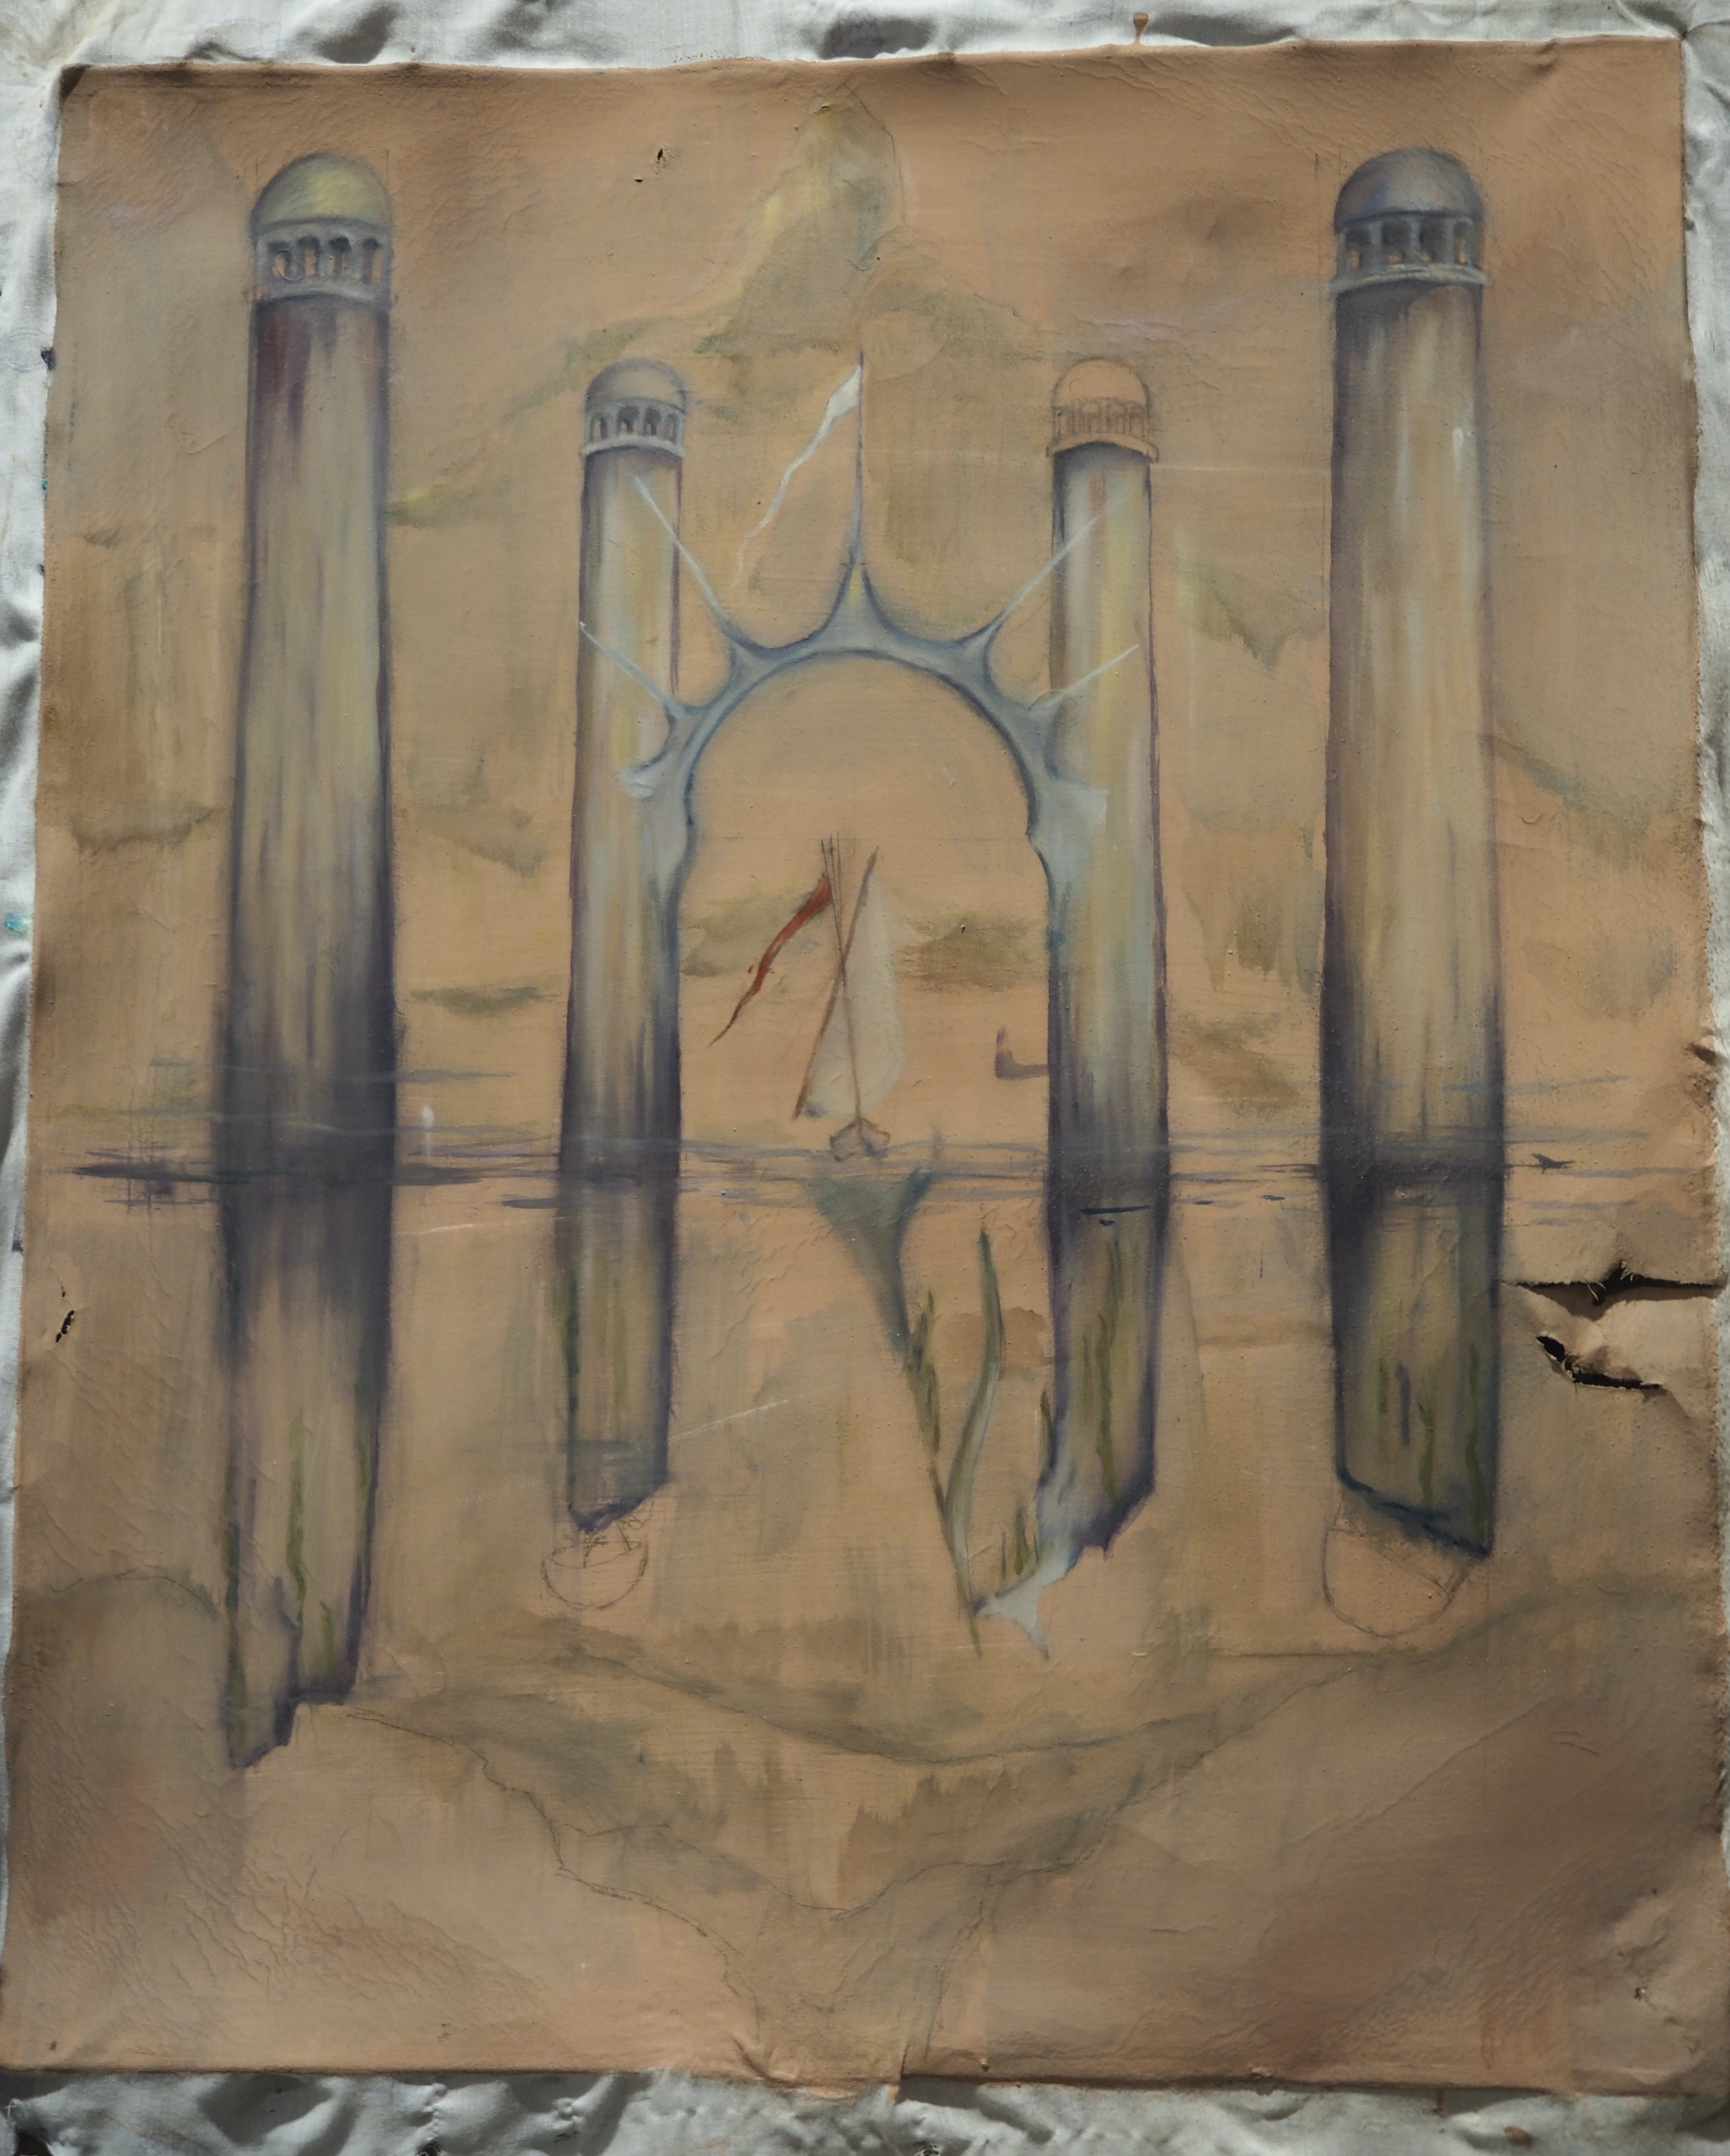
\includegraphics[scale=0.12]{/Users/rserrano/grepos/ProyectoFinal/_1010243.jpeg}
    \caption{El Cambio}
    \centering
  \end{figure*}

  
\item
  \emph{El No-Lugar} (Temple sobre tabla y óleo sobre tabla)
  
  Esta serie de tres obras intenta relfejar los no-lugares desde el
  punto de vista de la imagen y desde el del proceso: visualmente, se
  presentan como paisajes desolados, agrestes y hostiles, incompatibles
  con la vida en sociedad; procedimentalmente son abstracciones, pues no
  tenía intención representativa ni mimética al pintarlos, sólo de
  experimentar con la técnica y el
  color.
  \begin{figure*}
    \centering
    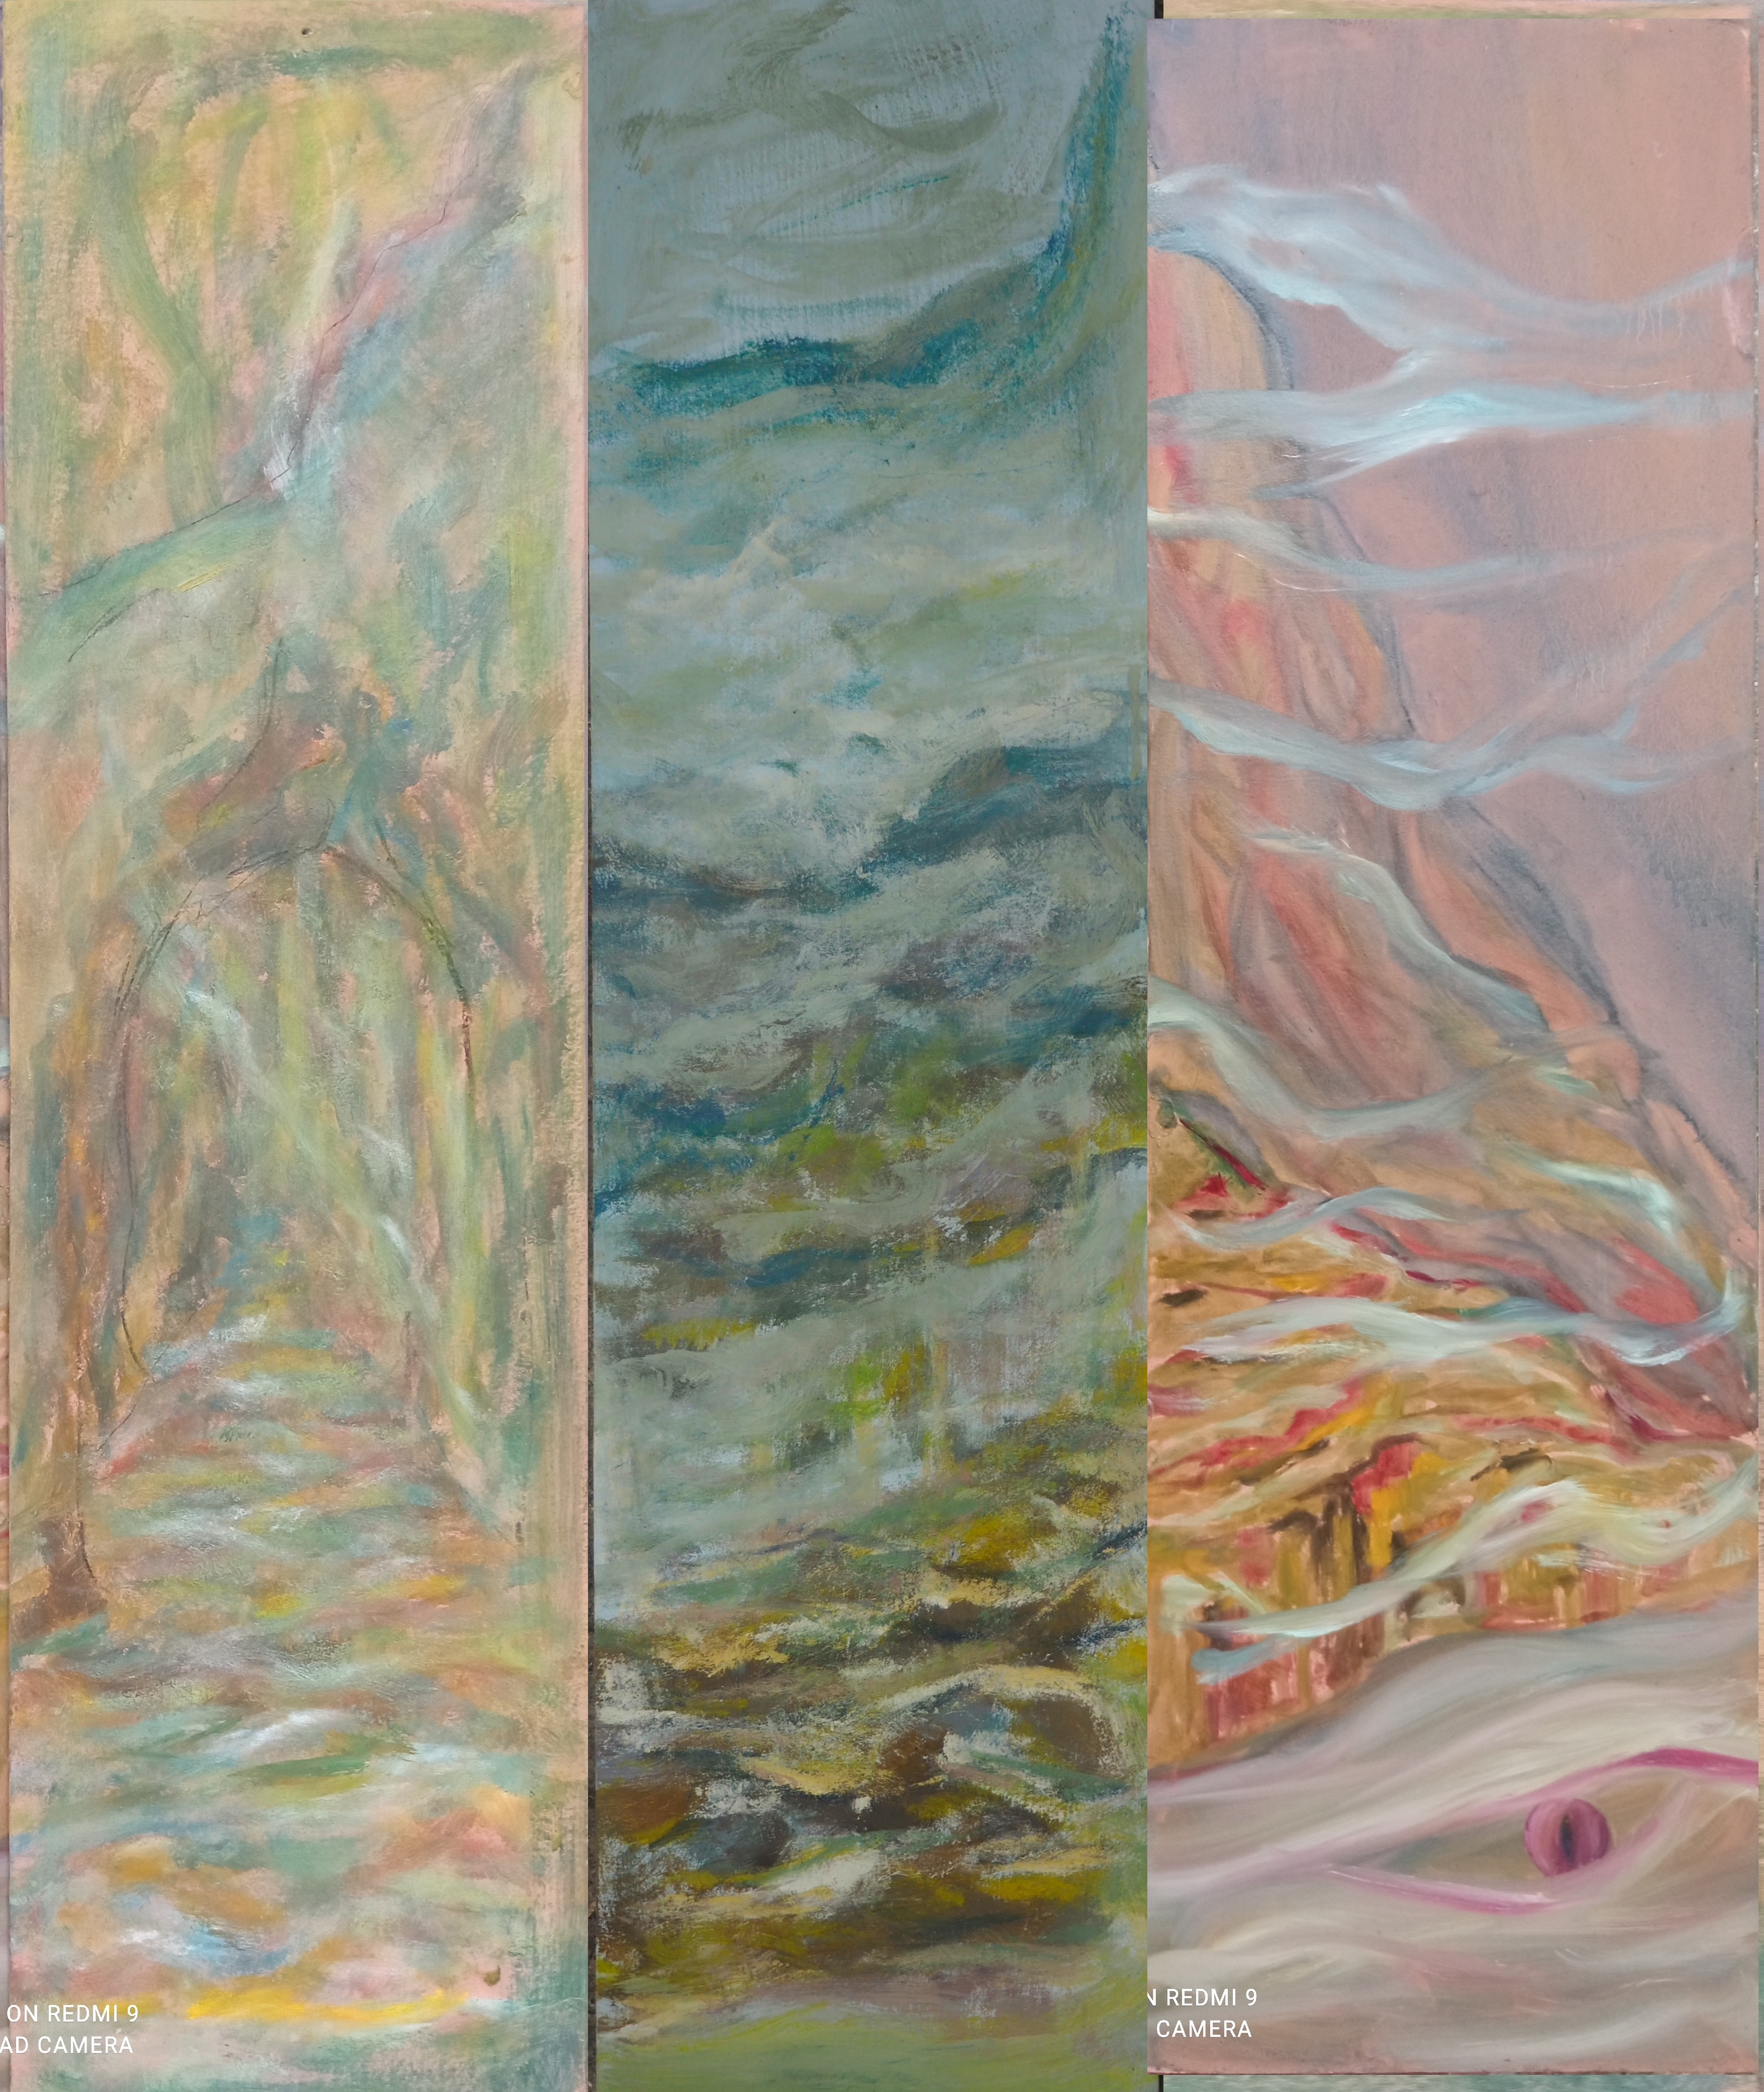
\includegraphics[scale=0.12]{/Users/rserrano/grepos/ProyectoFinal/Tabla1.jpg}
    \caption{El No-Lugar}
  \end{figure*}
  
\end{enumerate}

Otras obras que considero incluidas dentro del recorrido del proyecto,
aunque no son parte propiamente del mismo, están presentes en mi
esquina.

\hypertarget{anuxe1lisis-de-datos}{%
\subsection{Análisis de Datos}\label{anuxe1lisis-de-datos}}

Observando el recorrido, hasta ahora, del proyecto, creo que tengo claro
qué tipo de obra y procedimientos funcionan bien: la simplicidad en la
representación es clave para crear obras rápidas y efectivas, y creo que
es la manera con la que mejor consigo enseñar el mundo que voy creando
sobre la marcha.

En esta categoría se encuentran, en mi opinión, las arquitecturas y los
paisajes que he ido creando. Las arquitecturas complejas, aunque me
parece que funcionan, creo que se adecúan más a un dibujo esquemático y
un color plano y sencillo, en todo caso. Los intentos de hacer pintura
de estos dibujos creo que no dan el resultado esperado.

\clearpage

\hypertarget{conclusiones}{%
\section{Conclusiones}\label{conclusiones}}

En conclusión, estoy bastante satisfecho con la evolución de mi proyecto
personal durante este cuatrimestre, y creo que he desarrollado un estilo
y un lenguaje propios relativamente maduro.

\hypertarget{proyecto-final}{%
\subsection{Proyecto Final}\label{proyecto-final}}

Como proyecto final, he barajado varias ideas. La principal de ellas y
la que más me atrae es intentar rematar la creación de este mundo
fantástico empleando otra de mis pasiones a parte de la Pintura: la
informática.

\begin{figure}
  \centering
  \includegraphics[scale=0.24]{./davinci.jpeg}
  \caption{Páginas de un cuaderno de Da Vinci}
\end{figure}

Mi idea inicial era implementar un autómata\footnote{Un autómata celular
  (A.C.) es un modelo matemático y computacional para un sistema
  dinámico que evoluciona en pasos discretos. Es adecuado para modelar
  sistemas naturales que puedan ser descritos como una colección masiva
  de objetos simples que interactúen localmente unos con otros (desde
  Wikipedia:
  \url{https://es.wikipedia.org/wiki/Aut\%C3\%B3mata_celular}).} celular, cuyos patrones fueran interesantes y desarrollasen una gama
cromática parecida a la que uso en mi obra. Este autómata sería la
representación del mundo microscópico del mundo fantástico, en el que se
definen las interacciones básicas de este, y a partir de las cuales todo
es creado. Este sería el acto más elevado de creación pues,
virtualmente, sería posible crear todo a partir de estos bloques
básicos.

Esta idea, aunque muy interesante, se apoya poco en la pintura, y puede
llegar a ser complicada de realizar si surgiera algún problema.

Mi plan para el proyecto final se apoya en esta idea, pero incluye los
aspectos materiales y los procedimientos con los que he ido trabajando a
lo largo del cuatrimestre: definir, a la manera de los antiguos
filósofos griegos, una suerte de metafísica o cosmología para mi mundo,
y plasmarla en un documento hecho a mano, con bocetos, manuscrito, algo
parecido a los cuadernos de Da Vinci, o los códices medievales.\\

    %----------------------------------------------------------------------------------------

\end{document}
